\subsection{Translational Model}
\begin{frame}{Model}{Translational Model}	
    \only<1>{
        \begin{figure}[H]
            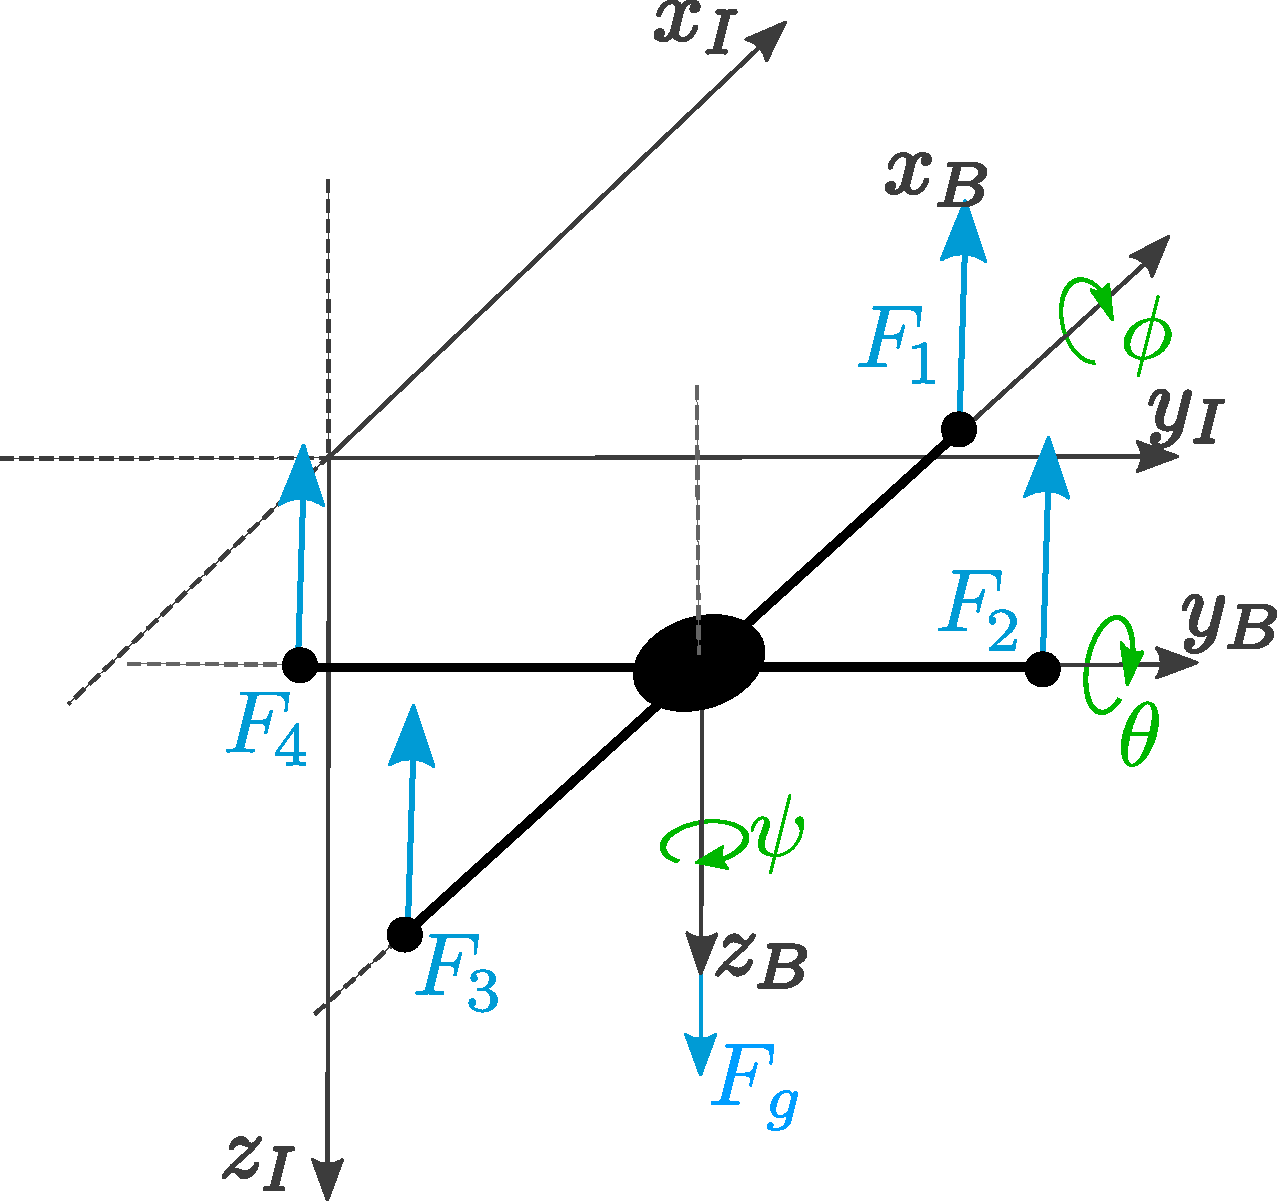
\includegraphics[width=0.6\textwidth]{figures/droneDiagramforcesup1}
        \end{figure}            
    }
    \only<2>{
        \begin{figure}[H]
            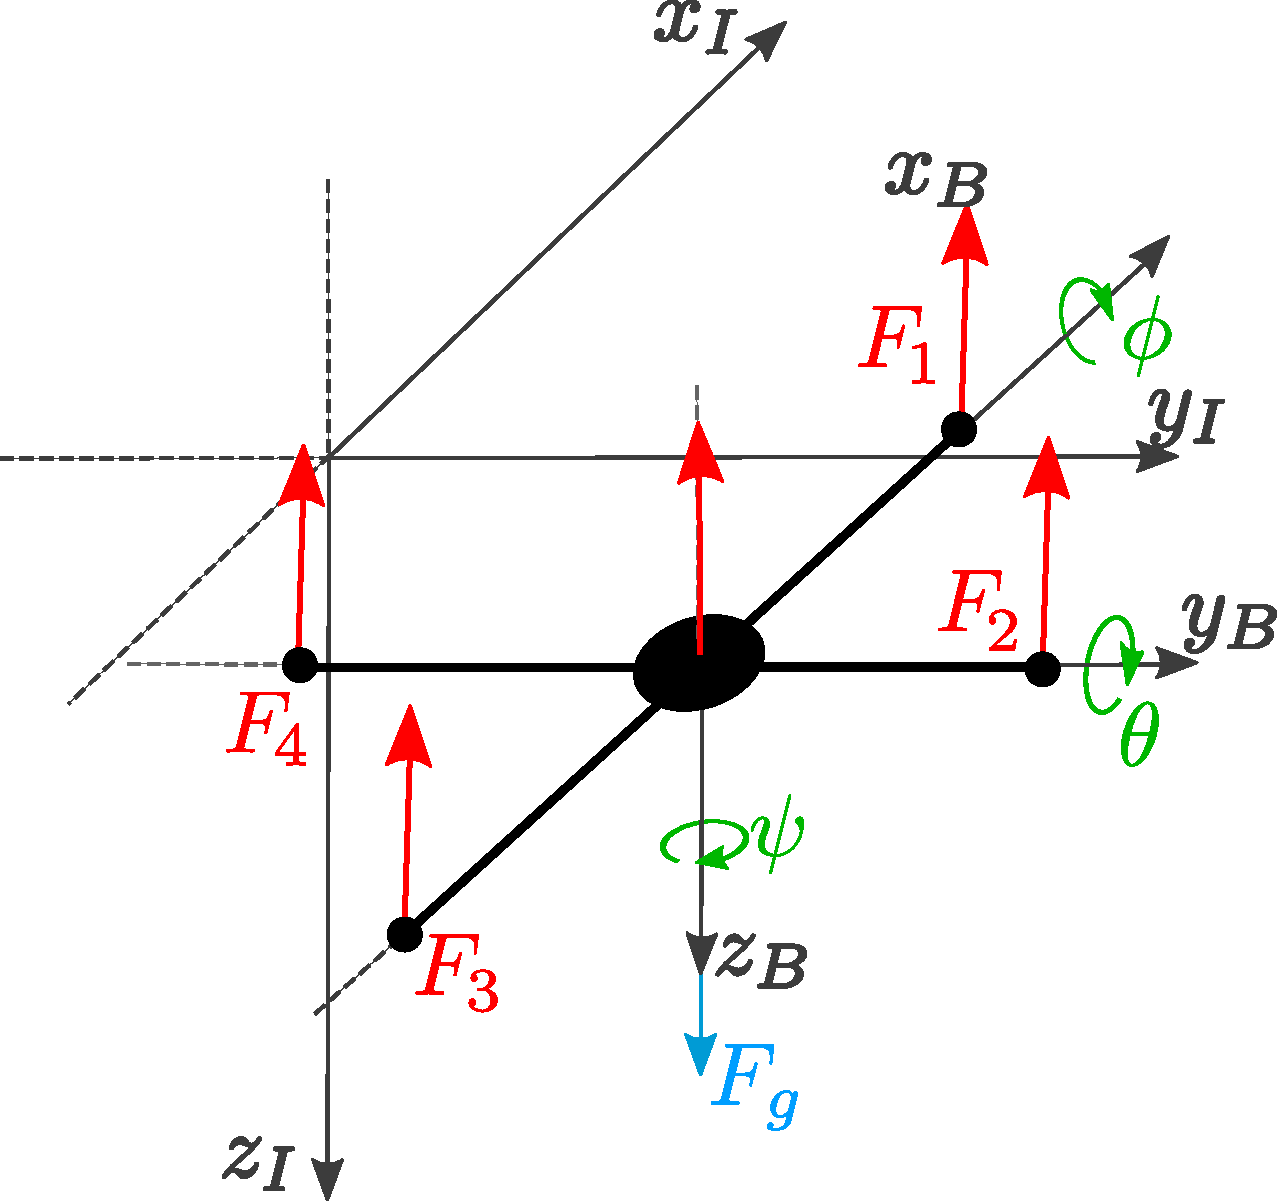
\includegraphics[width=0.6\textwidth]{figures/droneDiagramforcesup3}
        \end{figure}            
    }
    \only<3>{
        \begin{figure}[H]
            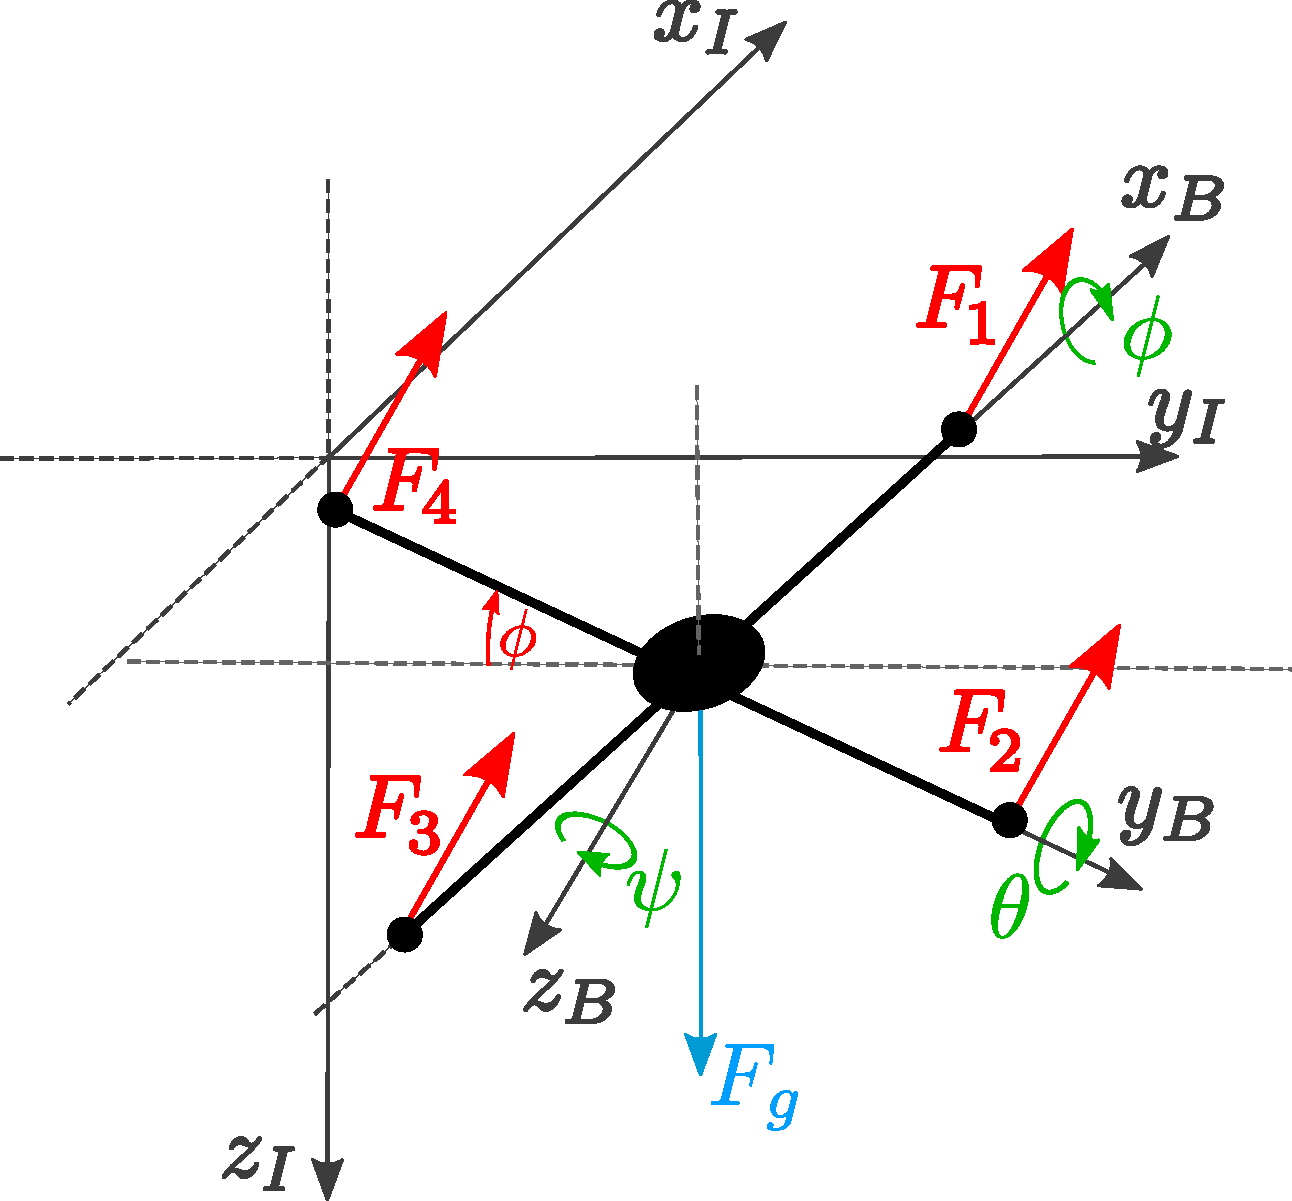
\includegraphics[width=0.6\textwidth]{figures/droneDiagramforcesuptilted}
        \end{figure}            
    }
    \only<4>{
        \begin{figure}[H]
            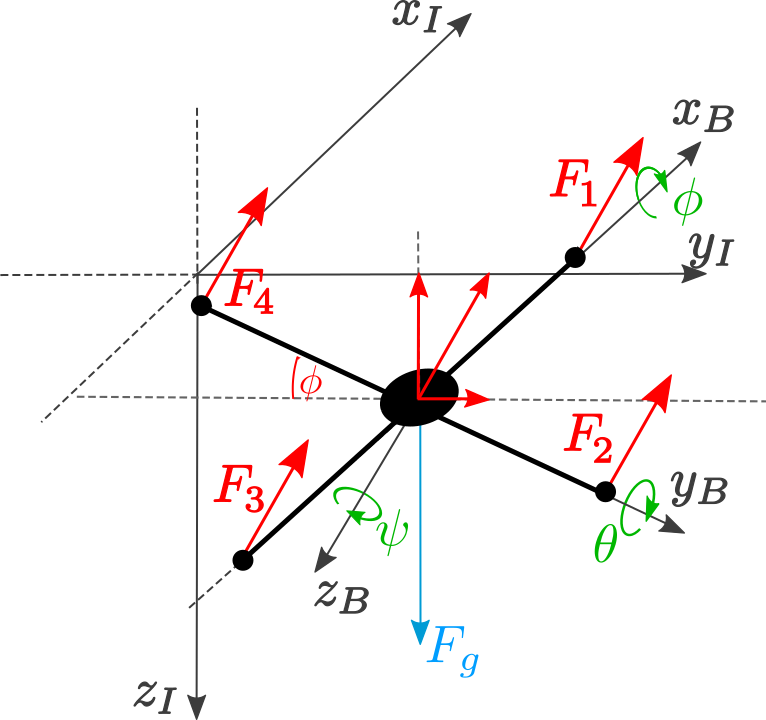
\includegraphics[width=0.6\textwidth]{figures/droneDiagramforcesuptiltedwithdecomposition}
        \end{figure}            
    }
\end{frame}

\begin{frame}{Translational Model}{}
    \begin{itemize}
        \item Rotation Matrix
    \end{itemize}
    
    \begin{minipage}{0.32\linewidth}
        \begin{flalign}
        R_X &=
        \begin{bmatrix}
        1 & 0        & 0         \\ 
        0 & c\phi  & -s\phi  \\ 
        0 & s\phi  & c\phi   \nonumber  
        \end{bmatrix} 
        \end{flalign}
    \end{minipage}\hfill
    \begin{minipage}{0.32\linewidth}
        \begin{flalign}
        R_Y &=
        \begin{bmatrix}
        c\theta  & 0  & s\theta  \\ 
        0          & 1  & 0          \\ 
        -s\theta & 0  & c\theta  \nonumber 
        \end{bmatrix} 
        \end{flalign}
    \end{minipage}\hfill
    \begin{minipage}{0.32\linewidth}
        \begin{flalign}
        R_Z &=
        \begin{bmatrix}
        c\psi & -s\psi  & 0  \\ 
        s\psi & c\psi   & 0  \\ 
        0       & 0         & 1  \nonumber 
        \end{bmatrix} 
        \end{flalign}
    \end{minipage}\hfill \\
    
    \vspace{0.7cm}
    
    \begin{flalign}
        R = R_Z R_Y R_X \nonumber
    \end{flalign}
    
    \begin{flalign}
        v_{\mathrm{I}}=Rv_\mathrm{B} \nonumber
    \end{flalign}
    
\end{frame}

\begin{frame}{Model}{Translational Model}
     \begin{itemize}
         \item Dynamic Equations
        \end{itemize}
        \uncover<2-4>{            
            \begin{flalign}
            m a=\sum F \nonumber
            \end{flalign}
        }
        \uncover<3-4>{
    \begin{flalign}
    m \ddot{x}_{\mathrm{I}} &= -(F_1+F_2+F_3+F_4) (\cos\phi \sin\theta \cos\psi + \sin\phi \sin\psi)  \nonumber\\
    m \ddot{y}_{\mathrm{I}} &= -(F_1+F_2+F_3+F_4) (\cos\phi \sin\theta \sin\psi - \sin\phi \cos\psi) \nonumber \\
    m \ddot{z}_{\mathrm{I}} &= F_g-(F_1+F_2+F_3+F_4) \cos\phi \cos\theta \nonumber
    \end{flalign}
    }
    \uncover<4>{
    \begin{flalign}
    m \ddot{x}_{\mathrm{I}} &= -k_{\mathrm{th}} ({\omega_1}^2+{\omega_2}^2+{\omega_3}^2+{\omega_4}^2) (\cos\phi \sin\theta \cos\psi + \sin\phi \sin\psi)   \nonumber\\
    m \ddot{y}_{\mathrm{I}} &= -k_{\mathrm{th}} ({\omega_1}^2+{\omega_2}^2+{\omega_3}^2+{\omega_4}^2) (\cos\phi \sin\theta \sin\psi - \sin\phi \cos\psi)  \nonumber\\
    m \ddot{z}_{\mathrm{I}} &= F_g-k_{\mathrm{th}} ({\omega_1}^2+{\omega_2}^2+{\omega_3}^2+{\omega_4}^2) \cos\phi \cos\theta
    \nonumber
    \end{flalign}
    }   
\end{frame}

\subsection{Linearization}
\begin{frame}{Model}{Linearization}
    \begin{itemize}
        \item First order Taylor approximation
    \end{itemize}
\uncover<2-4>{
  \begin{flalign}
  m \overline{\ddot{z}}_{\mathrm{I}} &= F_g-k_{\mathrm{th}} ({\overline{\omega}_1}^2+{\overline{\omega}_2}^2+{\overline{\omega}_3}^2+{\overline{\omega}_4}^2) \cos\overline{\phi} \cos\overline{\theta} \nonumber
  \end{flalign}  
}
\uncover<3-4>{
\begin{flalign}
\overline{\omega}_i=\sqrt{\frac{F_\mathrm{g}}{4k_{th}}}
\nonumber
\end{flalign}
}

\uncover<4>{
    \begin{minipage}{\linewidth}
        \begin{minipage}{0.5\linewidth}
       \begin{figure}[H]
           \centering
           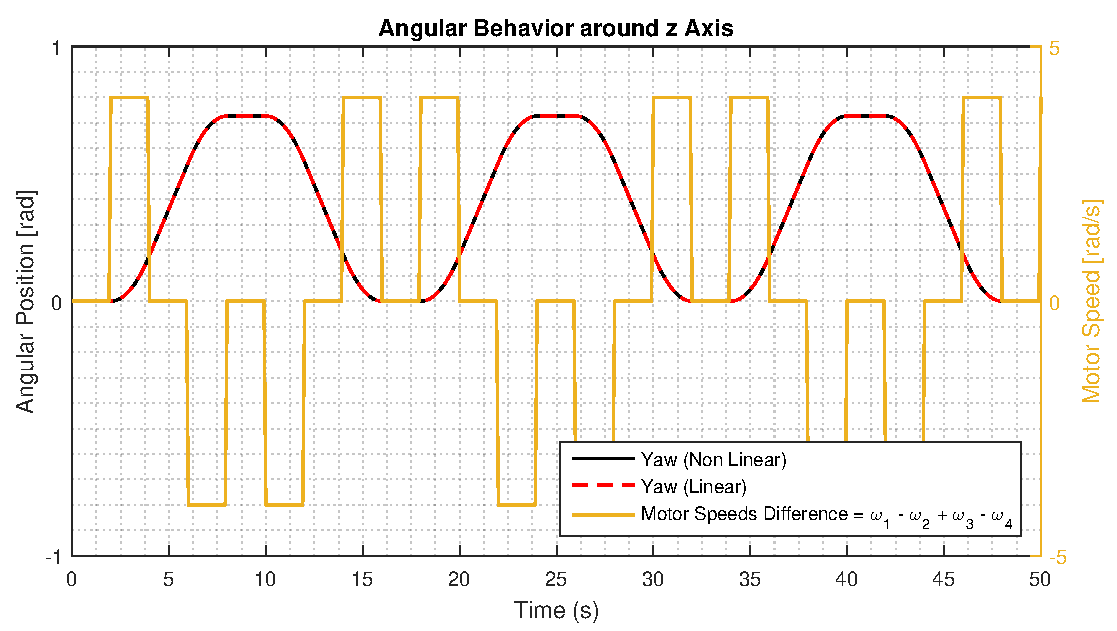
\includegraphics[width=\textwidth]{figures/yawCompModel}
        \end{figure}            
        \end{minipage}
        \hspace{0.03\linewidth}
        \begin{minipage}{0.5\linewidth}
       \begin{figure}[H]
           \centering
           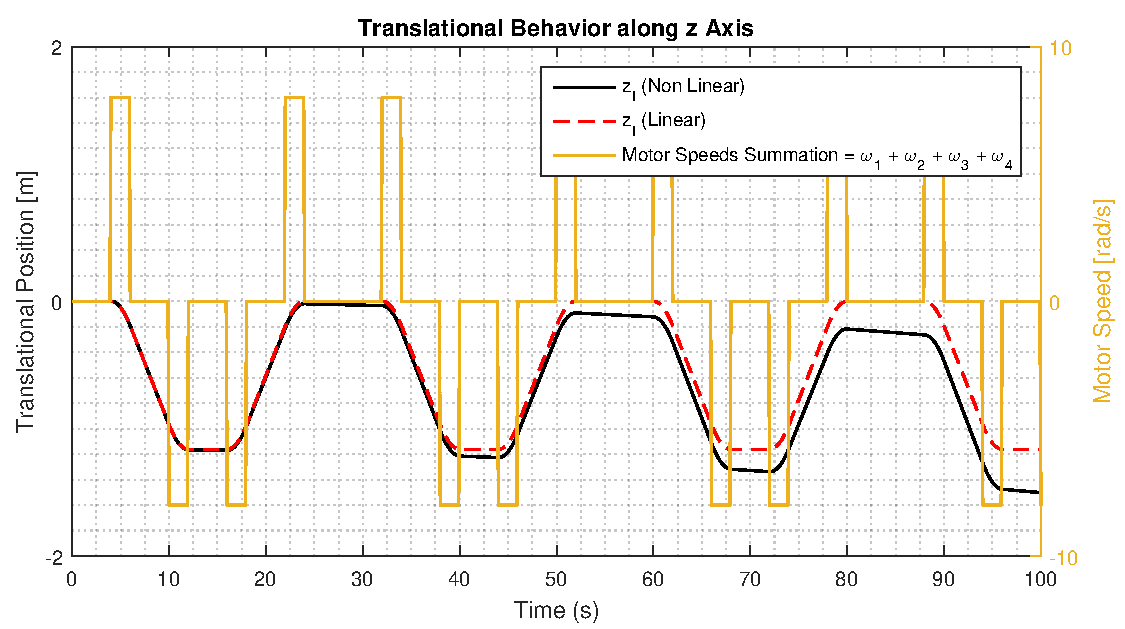
\includegraphics[width=\textwidth]{figures/zCompModel}
        \end{figure}          
    \end{minipage}        
    \end{minipage}
}
\end{frame}


%%%%%%%%%%%%%%%%
\section{Network}
\begin{frame}{Network}{}
   \begin{figure}
       \centering
        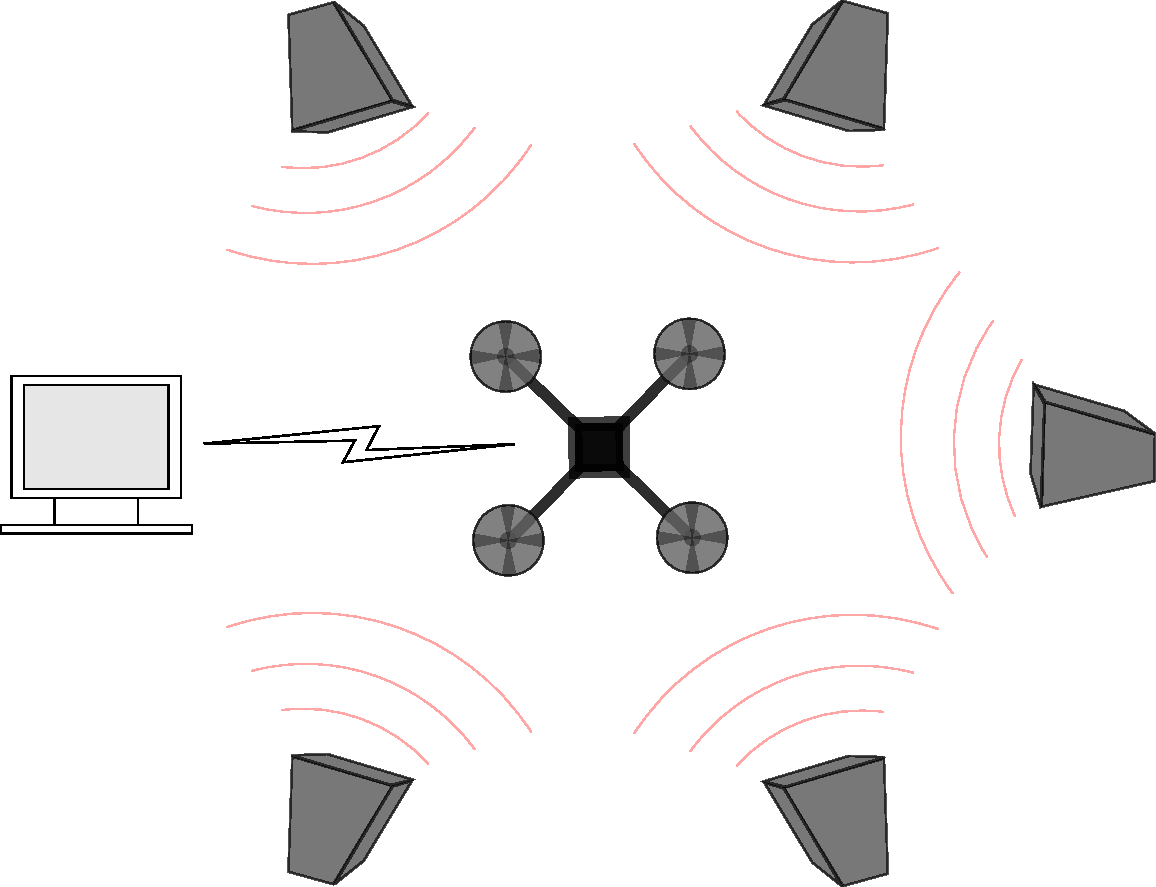
\includegraphics[width=0.5\linewidth]{figures/system.pdf}
    \end{figure} 

    \uncover<2>{
    \begin{itemize}
        \item Delay
    \end{itemize}
    \begin{itemize}
        \item Missed packets
    \end{itemize}
    }
    
\end{frame}

\begin{frame}{Network}{}
    
    \begin{minipage}{\linewidth}
        \begin{minipage}{0.49\linewidth}
            \begin{figure}[H]
                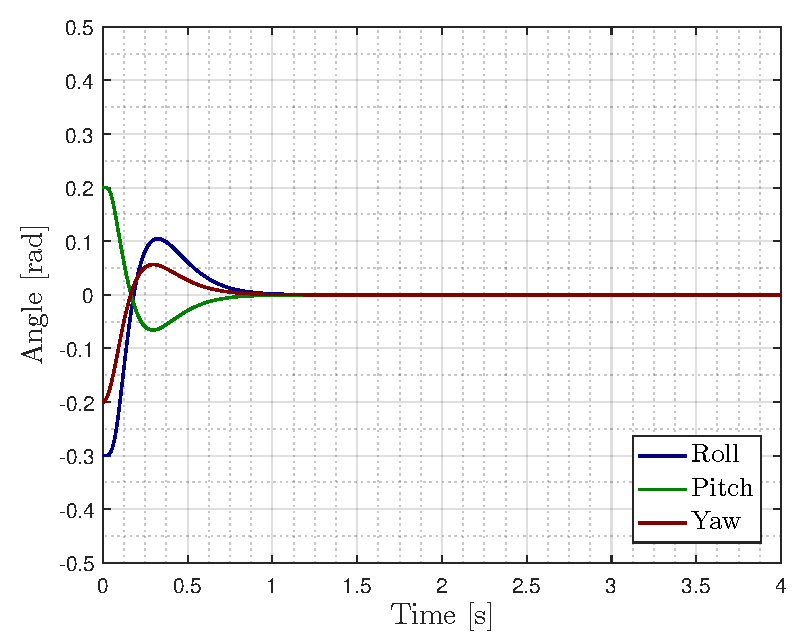
\includegraphics[width=1\textwidth]{figures/nonetwork}
            \end{figure}
            \centering
            Control design only taking the model into account
        \end{minipage}
        \hspace{0.03\linewidth}
        \begin{minipage}{0.49\linewidth}
            \begin{figure}[H]
                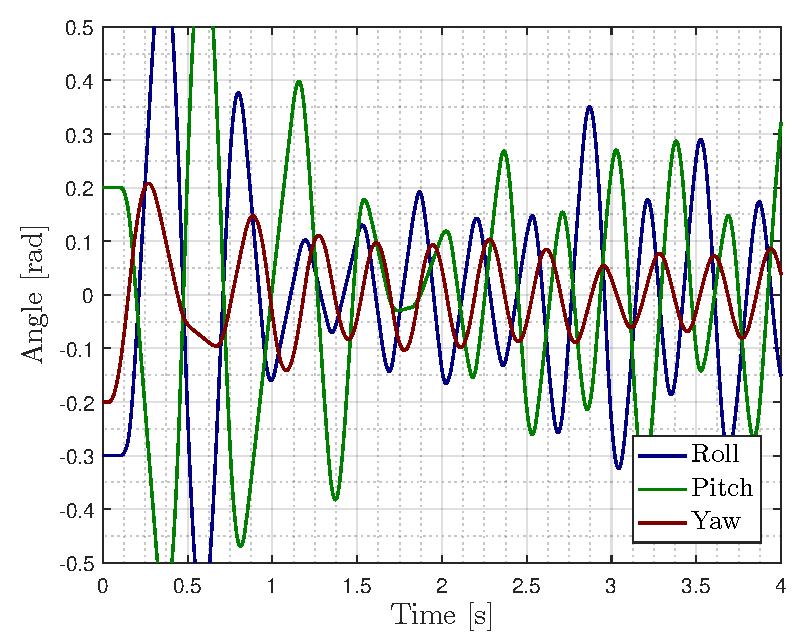
\includegraphics[width=1\textwidth]{figures/network}
            \end{figure}  
            \centering
            Same controller with the effect of the network                   
        \end{minipage}
    \end{minipage}  
\end{frame}

%%
% TOC
\begin{frame}{Agenda}{}
    \tableofcontents
\end{frame}

%%